\chapter{Čísla, znaky, reťazce}
\label{sect:cisla}

Doteraz sme hovorili, že typ \prg!int! obsahuje celé čísla. Je to ale trošku zložitejšie.
Skús si napísať takýto program:\\

\begin{lstlisting}
#include <iostream>
using namespace std;
int main() {
  int i, n = 1000;
  for (i = 0; i < 20; i++) {
    cout << n << endl;
    n = 10 * n;
  }
}
\end{lstlisting}


Čo sa deje? Zo začiatku program vypisuje vždy desaťnásobky čísla, tak ako by si čakal:
\vb{1000, 10000, 100000, \ldots}. Po čase sa ale namiesto násobkov desiatky začnú objavovať
čudné čísla. Prečo? Súvisí to s tým, ako sú čísla v počítači uložené. Pamäť sa skladá
zo súčiastok, ktoré môžu byť zapnuté alebo vypnuté, takže celá pamäť počítača sa dá predstaviť
ako véééľmi dlhé pole premenných, z ktorých každá môže byť 0 alebo 1. Takéto premenné
sa volajú {\em bity}. Keď chceme zapísať iné číslo ako 0 alebo 1, musíme ho uložiť
do viacerých bitov. Robíme to pomocou dvojkovej sústavy.

\indexItem{Mat}{dvojková a šestnástková sústava}
Keď zapisujeme čísla, spravidla to robíme v desiatkovej sústave. Pre čísla $0$ až $9$
máme znaky (číslice). Keď potrebujeme zapísať desiatku, na ktorú už nemáme znak, zabalíme
desať jednotiek do jedného balíka a počítame počet balíkov. Číslo $42$ teda znamená 
\cmd{štyri balíky po desať a ešte dve}. Keď sa nám minú číslice pre balíky, začneme
robiť balíky balíkov; počítame stovky a tak ďalej. My to robíme 
po desať, ale to isté môžeme robiť s akýmkoľvek číslom. Keď to budeme robiť s dvojkou\footnote{\phantomsection\label{foot:hexa}%
Často sa používa aj $16$-ková (tzv. hexadecimálna) sústava, kde mám číslice $0,1,2,\ldots,8,9,\mathrm{a,b,c,d,e,f}$, 
takže  \hbox{$\mathrm a_{16}=(10)_{10}$,} \hbox{$\mathrm b_{16}=(11)_{10}$,} \hbox{až $\mathrm f_{16}=(15)_{10}$}
a počítam so základom $16$, napr. $(\mathrm{beef})_{16}=$
\hbox{$\mathrm b_{16}\cdot 16^3+\mathrm e_{16}\cdot16^2+\mathrm e_{16}\cdot16+\mathrm f_{16}=$}
$11\cdot16^3+14\cdot16^2+14\cdot16+15=(48879)_{10}$.
V C++ môžeš priamo písať číslo v $16$-kovej sústave, ak pred neho napíšeš \vb{0x}. Napr. 
\vb{0xff} je \vb{255} a \hbox{\vb{0xfeeddadbeef} je \vb{17518595784431}}.
},
budeme namiesto balíkov po desať robiť balíky po dvoch. Teda budeme počítať $0$, $1$,
potm $10$ (t.j. \cmd{jeden balík po dvoch a nič iné}), $11$, $100$ (t.j. 
\cmd{jeden balík po štyroch a nič iné}), $101$, $110$, $111$ (t.j.
jeden balík po štyroch, jeden balík po dvoch a ešte jedna), $1000$, atď.
Napr. číslo $90$ zapíšeme v dvojkovej sústave $1011010$, pretože
$90=1\cdot64+0\cdot32+1\cdot16+1\cdot8+0\cdot4+1\cdot2+0\cdot1$\\

\centerline{\begin{tikzpicture}
  \foreach \v/\p [count=\i] in { 1/64, 0/32, 1/16, 1/8, 0/4, 1/2, 0/1} {
    \draw[dotted, shorten <= 2ex, shorten >= 2ex] 
    (\i,0) node [color=green!70!black] {{\small \p}}
     -- (\i,-6ex) node {\v};
  }
\end{tikzpicture}}

Názvy premenných sú len vecou programu; v skompilovanej binárke sú inštrukcie pre procesor,
ktoré hovoria, ako sa majú meniť hodnoty na jednotlivých miestach v pamäti.
Miesto v pamäti sa volá {\em adresa}.\indexItem{Alg}{adresa}
Keď v programe napíšeš \prg!int x;! kompilátor si nájde nejaké voľné
miesto v pamäti, kde bude uložená
premenná \prg!x!, zapamätá si jej adresu, a potom 
kedykoľvek v programe napíšeš napr. \prg!x=a!, tak 
kompilátor do 
binárky zapíše
inštrukciu pre procesor, aby počas behu programu nastavil bity
v pamäti na mieste, kde je \prg!x! uložené, podľa dvojkového zápisu $a$. 
Problém je v tom, že rôzne veľké čísla 
majú rôzne dlhý zápis. Keby napr. za premennou \prg!x! mala byť uložená premenná
\prg!y!, jej adresa by sa počas behu programu menila podľa toho, aké veľké číslo
je v premennej \prg!x! práve uložené. To by bolo veľmi nepraktické. Preto sa to rieši tak,
že na každú premennú sa vyhradí fixná dĺžka.
Keby si napísal\\

\vbox{
\begin{lstlisting}[] 
int x = 5591, a[2], r = 6893;
a[0] = 6802;
a[1] = 6737;
\end{lstlisting}
}

a veľkosť \prg!int! by bola
16 bitov, v pamäti by to mohlo vyzerať napr. takto\footnote{%
  Keď sme hovorili o poliach, vravel som, že treba dávať pozor, aby si
  nepísal za koniec poľa. Keby si v tejto situácii napísal \prg!a[2]=55;!,
  prepísala by sa ti premenná \prg!r! a ty by si netušil, kde sa tá chyba nabrala.
  }\\

\centerline{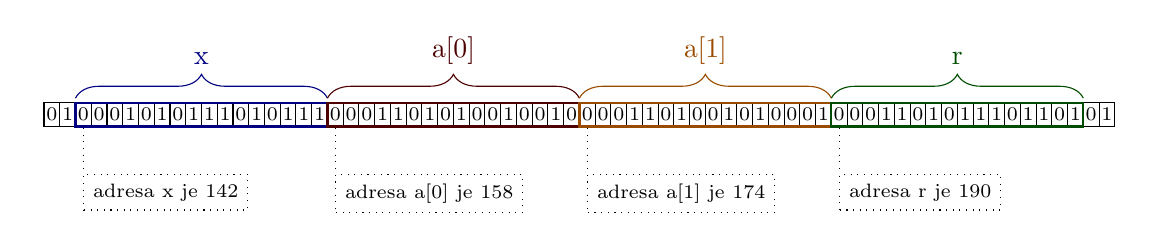
\begin{tikzpicture}[scale=0.2]
  \def\var#1#2#3{%
    \draw[#3] decorate[
       decoration={brace, amplitude=2ex}]{
       (#1,1.8) -- (#1+16,1.8) node [align=center,midway,anchor=south,yshift=2ex] {\vb{#2}}
        };
   \draw[#3,thick] (#1,0) rectangle (#1+16,1.5);

  }
  \foreach \v [count=\i] in {
    0,1,0,0,0,1,0,1,0,1,1,1,0,1,0,1,1,1,0,0,0,1,1,0,1,
    0,1,0,0,1,0,0,1,0,0,0,0,1,1,0,1,0,0,1,0,1,0,0,0,1,
    0,0,0,1,1,0,1,0,1,
    1,1,0,1,1,0,1,0,1
  }{
    \draw (\i,0) rectangle node [anchor=center] {{\scriptsize\roboto \v}} (\i+1,1.5);
  }
  \var3x{blue!50!black}
  \var{19}{a[0]}{red!30!black}
  \var{35}{a[1]}{orange!60!black}
  \var{51}{r}{green!30!black}

  \foreach \x/\v/\a in {3.5/x/142, 19.5/a[0]/158, 35.5/a[1]/174, 51.5/r/190 }{
  \draw[dotted] (\x,-0.1) -- (\x,-3) 
  node[draw, anchor = north west]{\scriptsize adresa \vb{\v} je \a};
  }

\end{tikzpicture}}

Skutočná veľkosť \prg!int! sa líši podľa systému, ale na väčšine súčasných počítačov je to 
32 bitov. Pretože prvý bit je vyhradený na znamienko ($+/-$), najväčšie číslo, aké
si môžeš v premennej typu \prg!int! zapamätať, je $1+2+2^2+2^3+\cdots+2^{30}=2147483647$.
Keby si sa pokúsil ešte pripočítať 1, prvý bit by sa nastavil na 1 a dostal by si záporné 
číslo. 

\indexItem{Prg}{typy \vb{long}, \vb{unsigned}, \vb{char}}
Preto existujú rôzne typy čísel: okrem \prg!int! je \prg!long!, ktorý je spravidla
dvakrát tak dlhý, t.j. má 64 bitov, takže najväčšie číslo je 
$1+2+2^2+\cdots+2^{62}=9223372036854775807$. Oba typy môžeš použiť vo verzii bez
znamienka (\prg!unsigned int!, \prg!unsigned long!) vtedy sa najväčšie číslo zdvojnásobí,
ale nedajú sa pamätať záporné čísla. Vyskúšaj si napísať\\

\vbox{
\begin{lstlisting}[] 
#include <iostream>
using namespace std;
int main() {
  unsigned int x = 0;
  cout << x << endl;
  x = x - 1;
  cout << x << endl;
}
\end{lstlisting}
}

Ako sa dá zapamätať text? Samozrejme, ako čísla. Máme typ \prg!char! (resp. 
\prg!unsigned char!) ktorý je dlhý 8 bitov (t.j. 1 byte). Funguje rovnako ako
typ \prg!int!. Každý znak anglickej abecedy má priradenú číselnú hodnotu podľa 
\indexItem{Alg}{ASCII}
\link{http://www.csc.villanova.edu/~tway/resources/ascii-table.html}{ASCII tabuľky}.
V programe sa dá použiť buď príslušné číslo, alebo znak v apostrofoch.
Keď máš premennú \prg!char x;! tak \prg!x=107;! a \prg!x='k';! urobia to isté.
Keďže je to číslo, dá sa s ním normálne rátať, napr. \prg!'a'+3=='d'! je \prg!true!.

\indexItem{Prg}{string, t.j. reťazec znakov}
Text sa pamätá ako pole znakov, napr. \prg!char hero[8];! Textu, zloženému
zo znakov, sa zvykne hovoriť {\em reťazec} ({\em string}). Príkaz na vypísanie,
\prg!cout<<! za normálnych okolností neakceptuje polia, ale pre pole znakov má výnimku
a vypíše ho ako text. Takisto, zadávať hodnoty \prg!hero[0]=71;! \prg!hero[1]=97;!\ldots
je nepraktické, preto existuje výnimka: pri vyrábaní poľa znakov sa dá priamo
inicializovať textom, napr. \prg!char hero[8]="Gandalf";! vyrobí pole\\

\centerline{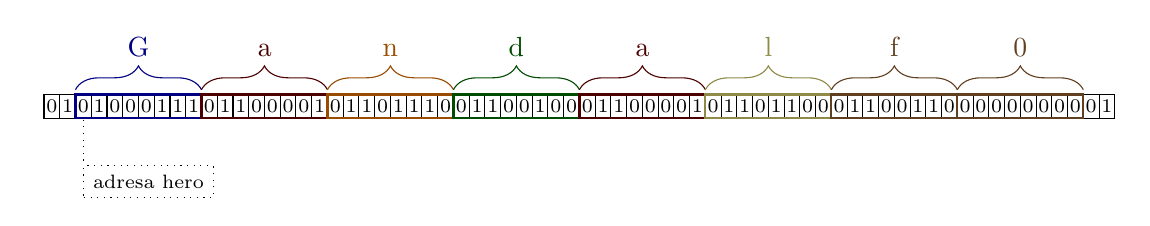
\begin{tikzpicture}[scale=0.2]
  \def\var#1#2#3{%
    \draw[#3] decorate[
       decoration={brace, amplitude=2ex}]{
       (#1,1.8) -- (#1+8,1.8) node [align=center,midway,anchor=south,yshift=2ex] {\vb{#2}}
        };
   \draw[#3,thick] (#1,0) rectangle (#1+8,1.5);

  }
  \foreach \v [count=\i] in {
    0,1,
    0,1,0,0,0,1,1,1,
    0,1,1,0,0,0,0,1,
    0,1,1,0,1,1,1,0,
    0,1,1,0,0,1,0,0,
    0,1,1,0,0,0,0,1,
    0,1,1,0,1,1,0,0,
    0,1,1,0,0,1,1,0,
    0,0,0,0,0,0,0,0,
    0,1
  }{
    \draw (\i,0) rectangle node [anchor=center] {{\scriptsize\roboto \v}} (\i+1,1.5);
  }
  \var3G{blue!50!black}
  \var{11}a{red!30!black}
  \var{19}{n}{orange!60!black}
  \var{27}{d}{green!30!black}
  \var{35}a{red!30!black}
  \var{43}l{yellow!50!black}
  \var{51}f{brown!50!black}
  \var{59}{0}{brown!50!black}
  
  \draw[dotted] (3.5,-0.1) -- (3.5,-3) 
  node[draw, anchor = north west]{\scriptsize adresa \vb{hero}};
\end{tikzpicture}}

Je konvencia, že posledný znak reťazca je nula, tak sa ľahko
zabezpečí, že do poľa viem uložiť aj kratší text než
na aký bolo rezervované. 
Len treba myslieť na to, rezervovať pole aspoň
o 1 dlhšie ako najdlhší plánovaný reťazec. 
Pri priradení reťazca do poľa znakov sa dá dľžka poľa vynechať, ak napíšeš
\prg!char hero[]="Gandalf";!, pole \prg!hero! sa vyrobí s dĺžkou $8$.
Pre vypisovanie existuje aj skratka,
že do príkazu \prg!cout<<! sa napíše priamo reťazec v dvojitých úvodzovkách, napr:\\

\vbox{
\begin{lstlisting}[] 
#include <iostream>
using namespace std;
int main() {
  char hero[8] = "Gandalf";
  cout << hero << " is a hero" << endl;
}
\end{lstlisting}
}

Príkaz na vypisovanie vypisuje zaradom 
znaky a skončí, keď narazí na znak 0, takže môže vypísať aj kratšie reťazce.
Čo vypíše tento program?\\

\vbox{
\begin{lstlisting}[] 
#include <iostream>
using namespace std;
int main() {
  char hero[8] = "Gandalf";
  hero[2] = 0;
  cout << "Hero is " << hero << endl;
}
\end{lstlisting}
}

Priradenie do poľa znakov naraz sa dá ale urobiť iba pri jeho vytváraní, takže
napísať neskôr \prg!hero="Batman";! sa nedá.

S načítavaním textu zo vstupu je to podobné, môžeš napísať\\

\vbox{
\begin{lstlisting}[] 
char mojText[20];
cin >> mojText;
\end{lstlisting}
}

Zo vstupu sa začnú čítať znaky až po prvú medzeru, tab, alebo koniec riadku\footnote{%
  \indexItem{Alg}{whitespace}Znaky medzera, tabulátor a nový riadok sa volajú {\em whitespace}.
Toto je dôležité: \prg!cin>>! prestane na prvom whitespace znaku. Aj pri načítavaní
čísel sa whitespace znaky preskakujú, takže je jedno, či sú vstupné čísla oddelené
medzerami alebo koncami riadkov.
Iná je situácia, ak sa načítava typ \prg!char!, vtedy sa whitespace nepreskakuje.
}a budú
sa ukladať do poľa \vb{mojText}. Toto sa ale prudko neodporúča robiť, 
lebo ak je na vstupe viac znakov,
ako je dĺžka poľa, začnú sa prepisovať ďalšie premenné. Vyskúšaj si
písať rôzne vstupy do tohto programu:\\

\vbox{
\begin{lstlisting}[] 
#include <iostream>
using namespace std;
int main() {
  char mojText[5];
  char x = '!';
  cin >> mojText;
  cout << mojText << " " << x << endl;
}
\end{lstlisting}
}


\begin{tabular}{@{\hspace*{0pt}}l@{\hspace*{1cm}}lp{10cm}}
Vstup:&Výstup:\\
\vb{pes} & \vb{pes !} &  nič zvláštne \\
\vb{pes a macka} & \vb{pes !} &  pohoda, načítava sa po prvú medzeru \\
\vb{macka} & \vb{macka } &  znak 0 z konca reťazca prepísal premennú \prg!x!\\
\vb{ABCDEFG} & \vb{ABCDEFG F} &  vypisuje sa až po znak 0, premenná \prg!x!
je prepísaná šiestym znakom
\end{tabular}

Keď na vstupe napíšeš veľmi dlhý text, \indexItem{Alg}{Segmentation fault}
asi spôsobíš, že program skončí s chybou \vb{Segmentation fault}: to je chyba, 
keď sa program snaží písať do takej časti pamäte, kde nemá prístup.
Načítavanie reťazcov je teda lepšie riešiť inak, ale o tom budeme hovoriť neskôr.
Nateraz nám toto stačí.

\begin{uloha}
  Používateľ zadá číslo $n$, potom $n$ čísel.
  Cieľom je vypísať ''súčtovú pyramídu'',
napr.\\

\begin{column}{0.45}
Vstup:\\
\begin{outputBox}
6
1 2 3 4 5 6
\end{outputBox}
\end{column}
\hfill
\begin{column}{0.45}
Výstup:\\
\begin{outputBox}
1 2 3 4 5 6
3 5 7 9 11
8 12 16 20
20 28 36
48 64
112
\end{outputBox}
\end{column}
\end{uloha}


\begin{uloha}
  Na vstupe je najprv číslo $n$, ktoré udáva počet kôp. Potom nasleduje
  niekoľko príkazov. Príkaz sa skladá z kľúčového slova a prípadných parametrov.
  Príkazy môžu byť:

\begin{itemize}\itemsep=-1mm
    \item \textcolor{magenta}{\vb{pridaj} {\em kam koľko}} 
      pridá {\em koľko} na kopu číslo {\em kam}
    \item \textcolor{magenta}{\vb{uber} {\em odkiaľ koľko}}
      uberie {\em koľko} z kopy číslo {\em kam}
    \item \textcolor{magenta}{\vb{max?}}
      zisti, aká veľká je najväčšia kopa
    \item \textcolor{magenta}{\vb{koniec}}
      skonči načítavanie
\end{itemize}

  Napíšte program, ktorý načíta vstup a pri každom príkaze \vb{max?}
  vypíše veľkosť najväčšej kopy. Napr. 

\begin{column}{0.45}
Vstup:\\
\begin{outputBox}
3
pridaj 1 10
uber 1 6
max?
pridaj 2 7
pridaj 2 3
max?
koniec
\end{outputBox}
\end{column}
\hfill
\begin{column}{0.45}
Výstup:\\
\begin{outputBox}
4
10
\end{outputBox}
\end{column}
\end{uloha}

\begin{uloha}
  Na stole sú rôzne geometrické útvary: body, kruhy a úsečky.
  Napíš program, ktorý z opisu predmetov vyráta najmenší obdĺžnik (ktorého
  strany sú rovnobežné s okrajmi stola), v ktorom sú všetky útvary.
  Na začiatku vstupu je počet útvarov $n$, Nasleduje $n$ riadkov,
  každý z nich je jedna z možností

\begin{itemize}\itemsep=-1mm
    \item \textcolor{magenta}{\vb{bod} {\em x y}} 
      bod so súradnicami $[x,y]$
    \item \textcolor{magenta}{\vb{kruh} {\em x y r}}
      kruh so stredom v bode $[x,y]$ a polomerom $r$
    \item \textcolor{magenta}{\vb{usecka} $x_1$ $y_1$ $x_2$ $y_2$}
      úsečka z bodu $[x_1,y_1]$ do bodu $[x_2,y_2]$
\end{itemize}

\begin{column}{0.35}
Vstup:\\
\begin{outputBox}
8
kruh 5 5 3
usecka 1 2 3 4
kruh 7 8 2
kruh 4 3 2
bod 10 5
bod 11 3
usecka 3 3 14 9
kruh 16 5 2
\end{outputBox}

Výstup:\\
\begin{outputBox}
1 1 18 10
\end{outputBox}
\end{column}
\hfill
\begin{column}{0.55}

  \centerline{
  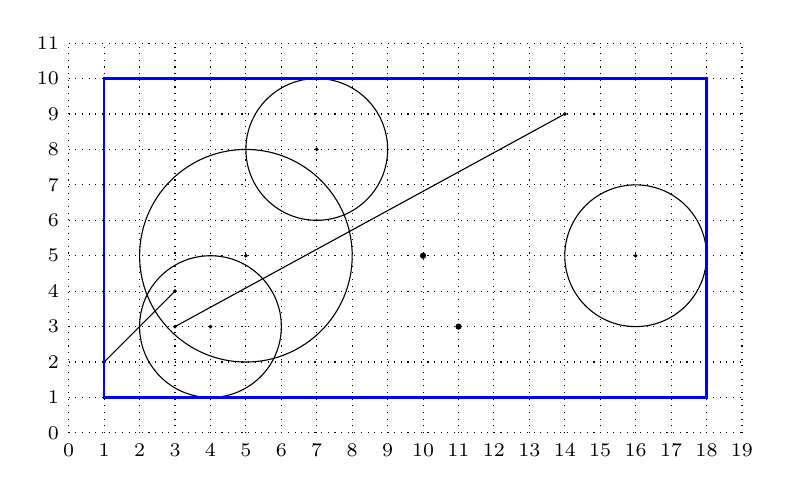
\begin{tikzpicture}[scale=0.45]
    \def\pp{1pt}
    \def\bb(#1,#2){;\filldraw(#1,#2) circle(2pt);}
    \def\cc(#1,#2)#3{\draw(#1,#2) circle (#3);\filldraw(#1,#2) circle(\pp);}
    \def\ll(#1,#2)(#3,#4){
      \draw(#1,#2) -- (#3,#4);
      \filldraw(#1,#2) circle(\pp);
      \filldraw(#3,#4) circle(\pp);
    }
    \draw[step=1.0,black,thin,dotted] (0,0) grid (19,11);
    \foreach \x in {0,...,19} {
      \node at (\x,-0.5) {{\scriptsize $\x$}};
    }
    \foreach \y in {0,...,11} {
      \node[anchor=east] at (0,\y) {{\scriptsize $\y$}};
    }
    \cc(5,5)3
    \ll(1,2)(3,4)
    \cc(7,8)2
    \cc(4,3)2
    \bb(10,5)
    \bb(11,3)
    \ll(3,3)(14,9)
    \cc(16,5)2
    \draw[blue,thick](1,1) rectangle (18,10);
  \end{tikzpicture}}
\end{column}
\end{uloha}
